\documentclass{article}


% if you need to pass options to natbib, use, e.g.:
%     \PassOptionsToPackage{numbers, compress}{natbib}
% before loading neurips_2021

% ready for submission
\PassOptionsToPackage{numbers, compress}{natbib}
\usepackage[preprint]{neurips_2021}
\bibliographystyle{abbrvnat}

\usepackage[utf8]{inputenc} % allow utf-8 input
\usepackage[T1]{fontenc}    % use 8-bit T1 fonts
\usepackage[colorlinks=true]{hyperref}       % hyperlinks
\usepackage{url}            % simple URL typesetting
\usepackage{booktabs}       % professional-quality tables
\usepackage{amsfonts}       % blackboard math symbols
\usepackage{nicefrac}       % compact symbols for 1/2, etc.
\usepackage{microtype}      % microtypography
\usepackage{xcolor}         % colors
\usepackage{siunitx}
\usepackage{graphicx}

\newcommand{\todo}[1]{{\color{red}todo: #1}}

\title{Spotify feat. Logistic Regression - \\ Popularity, Nothing Else Matters}

% The \author macro works with any number of authors. There are two commands
% used to separate the names and addresses of multiple authors: \And and \AND.
%
% Using \And between authors leaves it to LaTeX to determine where to break the
% lines. Using \AND forces a line break at that point. So, if LaTeX puts 3 of 4
% authors names on the first line, and the last on the second line, try using
% \AND instead of \And before the third author name.

\author{%
  Sebastian Hoffmann\thanks{correspondence to \texttt{sebastian.hoffmann@student.uni-tuebingen.de}}\\
  University of Tübingen\\
  Matriculation number 5954377\\
  \And
  Yannick Streicher\thanks{correspondence to \texttt{yannick.streicher@student.uni-tuebingen.de}}\\
  University of Tübingen\\
  Matriculation number 5331817\\
}

\begin{document}

\maketitle

\begin{abstract}
  What is the musical taste of the world? With the recent rise and global pervasiveness of music streaming services, such as Spotify, or Apple Music, answering this question has potentially become tractable. For this, we analyze a subset of 1.2 million songs scraped from Spotify that we further augment with popularity and genre information. While we find that the musical features extracted by Spotify are discriminative of the genre of a song, they are poor predictors of the popularity if used in a linear model, such as linear or logistic regression. Our results indicate that either more complex models are necessary or that the task itself is to some degree ill-posed, for instance due to a low signal-to-noise ratio.
\end{abstract}

\section{Introduction}
%
% Musical taste has historically always been changing. While Jazz has been highly popular throughout the 50s to 60s for instance, it has since then seen a steep decline and new trends, such as Funk, or Disco in the 70s, or Heavy Metal in the 80s, emerged. As songs within a genre often build upon the same musical foundation, e.g. the use of extended triads and swung-eigths in Jazz, this begs the question if the popularity of a song can be predicted from musical features alone.
%
With the recent advent of musical streaming services, such as Spotify, or Apple Music, unprecedented amounts of music data became readily available to the public. This data can often be accessed free-of-charge using an API provided by the provider of the service itself. Due to their large userbase, popularity measures derived from these platforms provide a robust measure, at least for their target demographics.

In this work we want to explore if the musical features extracted by Spotify for individual songs, such as tempo or key, can be used to predict  its popularity. We are particular interested in if this can be achieved using a simple linear model such as linear or logistic regression. This would allow direct interpretability of what musical properties a popular song possesses.
%
Furthermore, we are interested in how todays musical landscape is shaped. To this end, we analyze the distribution of genres of songs available on Spotify and investigate if there are some genres which are particular popular or unpopular.

\section{Dataset}
\label{sec:dataset}
%
While Spotify provides data about individual songs or artists via its API, it does, however, not provide a catalog of available songs on its platform. Thus, we use a dataset\footnote{\url{https://www.kaggle.com/rodolfofigueroa/spotify-12m-songs}} of $1.2$ million songs made available on Kaggle, a subset of the $70$ million songs accessible on Spotify~\cite{ingham_2020}. This dataset was created by first downloading the \href{https://musicbrainz.org/}{MusicBrainz} catalog, an open-collaboration database of music releases, and then querying the Spotify API. 

For each song listed, the dataset contains basic meta informations such as artist and song name, as well as a set of $14$ song features that are provided by Spotify. These features include, among others, the estimated tempo, key, energy, danceability, or duration of the song. For a full list, refer to the Spotify API documentation. Crucially, the popularity or genre of a song is not included in this dataset.

\subsection{Augmentation and Filtering}
In a first step we retrieve additional information of all \num{85 113} artists appearing in the dataset from the Spotify API. This information includes the popularity of that artist, aggregated from individual songs, the number of followers, and optionally a list of genres the artist is associated with.
%
Additionally, we query the Spotify API for every song in the dataset to obtain its individual popularity. While Spotify does not provide genre information at song level, we use the genre information associated with the first artist to further augment the dataset. The exact procedure is described in Section~\ref{sec:genre_clustering}. 
We further apply a filtering scheme based on PCA to only include professional or semi-professional musicians. Further details are given in the supplementary material on github\footnote{\url{https://github.com/ystreicher/SpotifyNEM2022}}.
In total, $62.8\%$ of all artists are removed from the dataset. This reduces the number of songs left in the dataset to \num{755472} ($62.75\%$).

% \subsection{Filtering}

%\begin{figure}[t]
%  \centering
%  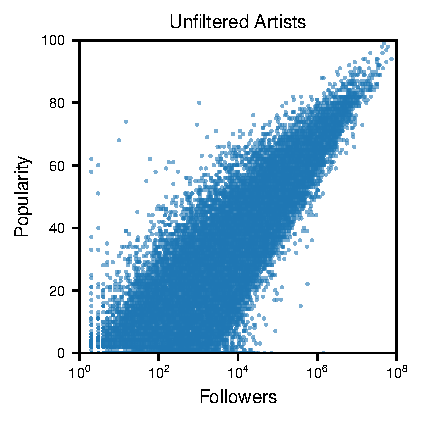
\includegraphics[width=0.38\textwidth]{../figures/artists_unfiltered.pdf}
%  \qquad
%  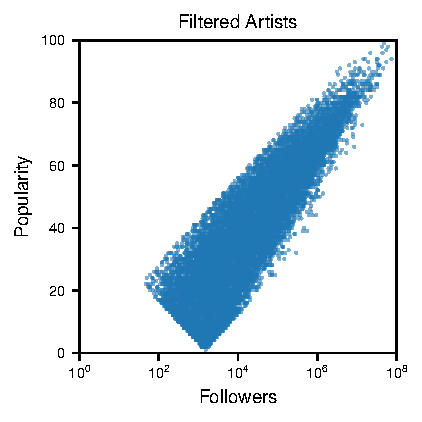
\includegraphics[width=0.38\textwidth]{../figures/artists_filtered.pdf}
%  \caption{\textit{Left}: Artist popularity against log-followers before applying our filtering rules. \textit{Right}: We use the result of PCA to exclude artists that are outliers with respect to the first and second principal component.}
%  \label{fig:filtering}
%\end{figure}

% To reduce potential noise introduced by unknown self-published artists, we want to restrict our analysis to those that can be considered professional or semi-professional musicians. This step was deemed necessary, as self-published artists do not undergo the feedback and quality control process a regular music label would provide. Indeed, we find that a quarter of artists on Spotify have less than $45$ followers and half of all artist have less than $393$.
% %For comparison, \emph{Merikan}, a relatively unknown Drum and Bass producer, has $4581$ follower at the time of writing.

% We find that the number of followers is roughly exponentially distributed. After applying a logarithmic transform, a clear linear relationship between the number of log-followers and popularity is visible (Pearson correlation coefficient: $0.88$). 
% %
% Based on the popularity and log-follower count, we derive a robust filter criterion using principal component analysis~(PCA)~\cite{jolliffe2016principal}. After applying PCA, the first principal component is treated as a measure of the successfulness of an artist, taking both his popularity and followers into account. We threshold this measure to only include $50\%$ of all artists. Furthermore, we threshold the second component as well to remove outliers, i.e. artists with a high discrepancy between popularity and follower count. This step affects $1.6\%$ of all artists. Finally, we exclude those without associated genres.

% In total, $62.8\%$ of all artists are removed from the dataset. This reduces the number of songs left in the dataset to $755472$ ($62.75\%$).

\subsection{Finding supergenres by clustering}
\label{sec:genre_clustering}
The genres associated with an artist are often finely granulated. Out of $4713$ genres in total, only $496$ have more than $50$ artists associated with them. To reduce the number of overall genres to a handful of overarching \emph{supergenres}, such as Rock, Jazz, or Hip-Hop, we employ agglomerative clustering~\cite{ward1963hierarchical} (we use~\cite{scikit-learn}). Agglomerative clustering lends itself naturally for this as it exploits the inherent hierachical relationship between genres.

Inspired by constrastive methods~\cite{mikolov2013efficient, chen2020simple}, we exploit the fact that related genres are more likely to be associated with the same artist to construct a distance measure. In a first step, a similarity measure $s_{i, j} = (2 n_{ij}) / (N_i + N_j)$ between the $i$-th and $j$-th genre is defined, where $n_{ij}$ denotes the number of times they appear together and $N_i, N_j$ the total counts of the $i$-th and $j$-th genre respectively. The distance can then be defined as the reciprocal of that similarity measure. We then use this distance measure for the clustering procedure.

By running the clustering algorithm on an aggressively filtered subset of genres, we find $32$ supergenres, among them Jazz, Classical, Metal, Rock, Pop, or EDM, but also Soundtrack, or Show Tunes\footnote{Supergenres have been manually annotated}. These cover $60.5\%$ of all songs in the filtered dataset. To further improve coverage of songs, we rerun the clustering with less aggressive filtering to include more fine-grained genres. We then manually append these additional subgenres to the appropriate supergenre if applicable. This improves coverage to $71.3\%$.

\section{Experiments}

\subsection{Genre analysis}

\begin{figure}
  \centering
  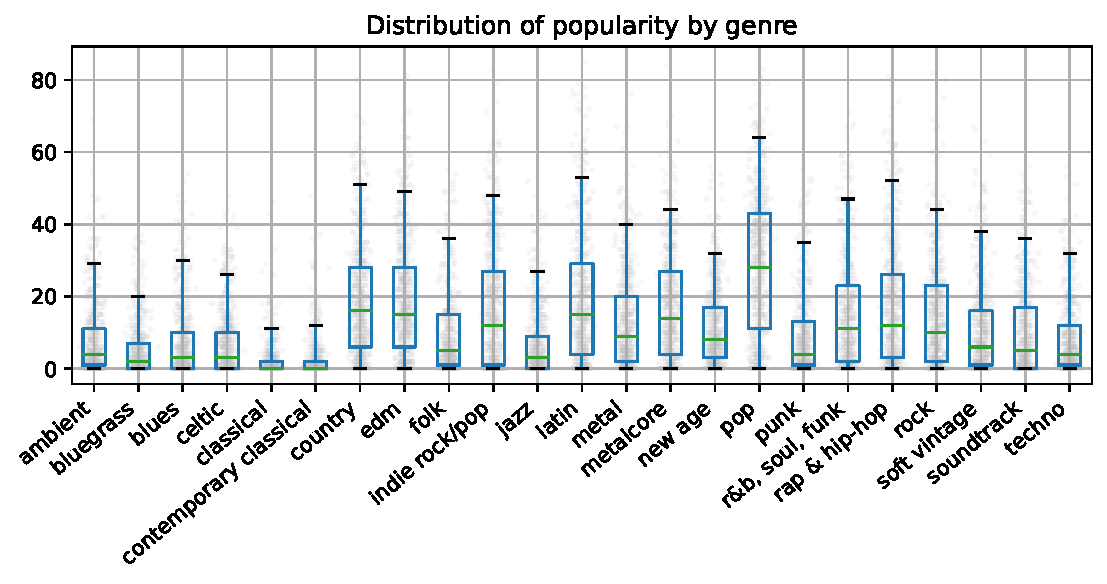
\includegraphics[width=0.85\textwidth]{../figures/popularity_distribution_by_genre.pdf}
  \caption{Box plot of popularity grouped by genre. Boxes span $Q1$ to $Q3$,while whiskers indicate the $5$-th and $95$-th percentile respectively. The central line shows the median of the distribution. Among all genres, Pop has the highest median and $95$-th percentile.}
  \label{fig:genre_boxplot}
\end{figure}

The most prelevant genre on Spotify is Classical ($20.6\%$), followed by Rock ($7.9\%$), Rap / Hip-Hop ($7.6\%$), Metal ($6.3\%$), Folk ($6.0\%$), and Jazz ($4.0\%$). For a complete listing, we refer to the supplementary material available on github\footnotemark[5].

The box plot presented in Fig.~\ref{fig:genre_boxplot} shows the distribution of popularity for each supergenre. We find that despite  being the most prominent genre, Clasical and Contempory Classical are by far the most unpopular with the majority of the probability mass below $10\%$. Notably, Pop has by far the heaviest tails and the highest median and $75$-th percentile of all genres despite only making up $2.9\%$ of all songs. Following after Pop, we find that Country, EDM, Latin, Rock, Indie Pop, Hip-Hop, and Metalcore are almost equally popular.

Lastly, as a preliminary experiment for the logistic regression, we investigate the discriminative power of the musical features provided by Spotify. For this, we embed the features of songs of the six most prominent genres into a two-dimensional vector space using t-SNE. Results are presented on github. Clearly visible are distinct cluster of songs corresponding to genres such as Hip-Hop, Metal, Classical or Jazz. Additionally, genres that are arguably to some extent similar, such as Rock and Metal, or Jazz and Classical, are clustered close together.

\subsection{Logistic Regression}
Before applying logistic regression, we test if popularity can be predicted using linear regression from the musical features (c.f.~Section~\ref{sec:dataset}) as a preliminary experiment. We obtain significant but small coefficients that can only explain about \SI{10}{\percent} of the variance in the data. Loudness appears to be the most important feature according to the model. We now investigate if logistic regression can be used to classify songs as either popular or unpopular. 

Binary labels are obtained by thresholding the popularity value of a song. Despite our aggressive filtering, we find that the popularity is roughly exponentially distributed. To deal with such a highly-skewed distribution, we try two thresholding strategies:
\begin{enumerate}
  \item[(A)] Any song with popularity below the $90$-th percentile is labelled \emph{unpopular}, otherwise as \emph{popular}. To counteract the class-imbalance, the class weights are adjusted.
  \item[(B)] The songs are evenly split into two classes at the $50$-th percentile.
\end{enumerate}

In all experiments an 80-20 train-test split is used, and $\ell_2$-regularizaton is employed in both cases. To find the optimal regularization strength, we performed a grid-search using 5-fold cross validation on the training set.

Overall, model A achieves an accuracy of $0.59$, whereas model B achieves an accuracy of $0.62$ w.r.t. to their respective labels.
A calibration plot is presented in Fig.~\ref{fig:logis_eval}~(left). 
Both models are poorly calibrated and possess higher mean $\ell_1$-loss than random guessing (not shown). Combined with the low $R^2$-score of the linear model, this might indicate that popularity can only be poorly predicted using a linear relationship. To test if a higher capacity model could potentially improve performance, we further train a simple multilayer perceptron, but report only marginally improved results.

Nevertheless, we show learned coefficients of model B in Fig.~\ref{fig:logis_eval} (right). In accordance with the linear regression, especially loudness and danceability seem to be indicative of popularity. In contrast, acousticness, instrumentalness, energy, and valence appear to have a negative impact.

\begin{figure}
  \centering
  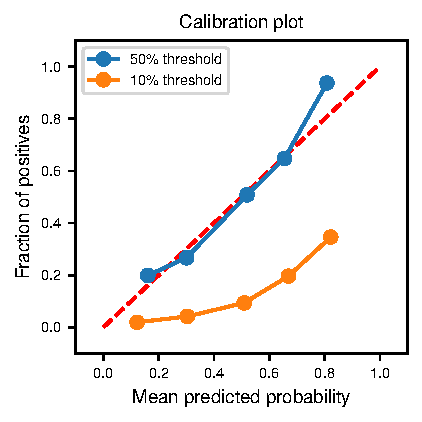
\includegraphics[width=0.39\textwidth]{../figures/calibration_combined.pdf}
  \qquad
  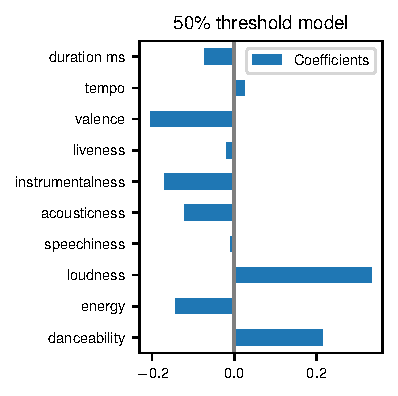
\includegraphics[width=0.39\textwidth]{../figures/logistic_coefs_50_threshold_model.pdf}
  \caption{\textit{Left}: Calibration plot. The prediction space is discretized into \num{20} bins. Using the test set, for each bin, we plot the fraction of true popular songs against the mean predicted probability for those songs. \textit{Right}: The coefficients of the selected model for each audio feature. For the interpretation of individual features consider the API documentation of Spotify.}
  \label{fig:logis_eval}
\end{figure}
  

\section{Conclusion}

In this work, we gave an overview of the musical landscape as seen by Spotify.
We demonstrated that agglomerative clustering can successfully be applied to aggregate the thousands of microgenres identified by Spotify's algorithm into a handful of supergenres. 
Furthermore, we have shown that the musical features provided by Spotify's API are highly discriminative in terms of \emph{musical relatedness} by applying t-SNE and showing that songs of the same genre are spatially close in  feature space. Despite some genres being less and more popular than others, we find linear models to be only poor predictors of the popularity of an individual song.

Contrary to previous results~\cite{viney2008obsession} ($n=30$), our experiments show that loudness correlates, albeit very weakly, with the popularity of a song. This does not necessarily imply a causation, however. Rather, it could be indicative of the previously recognized \emph{loudness war}~\cite{vickers2010loudness}. Either, because successful songs are more likely to have undergone a rigorous mixing and mastering process, or because more recently released songs, thus on-average louder songs, are more popular by construction of the metric.

Our results provide some evidence that the musical properties of a song might only have a minor impact on its popularity and commercial success. As previously recognized in the literature~\cite{viney2008obsession}, other factors not covered in the data, such as marketing efforts, or radio and television airplay might have a much bigger impact instead. Finally, it is not unreasonable to assume that popularity is inherently very noisy, i.e. dominated by chance.  

%The work allows two conclusions: Either, the crucial factors for popularity are not represented in the data set, or, higher capacity models are needed to solve the problem.


\bibliography{bibliography}

% \begin{appendix}
% \section{Appendix}

% \begin{figure}[h]
%   \centering
%   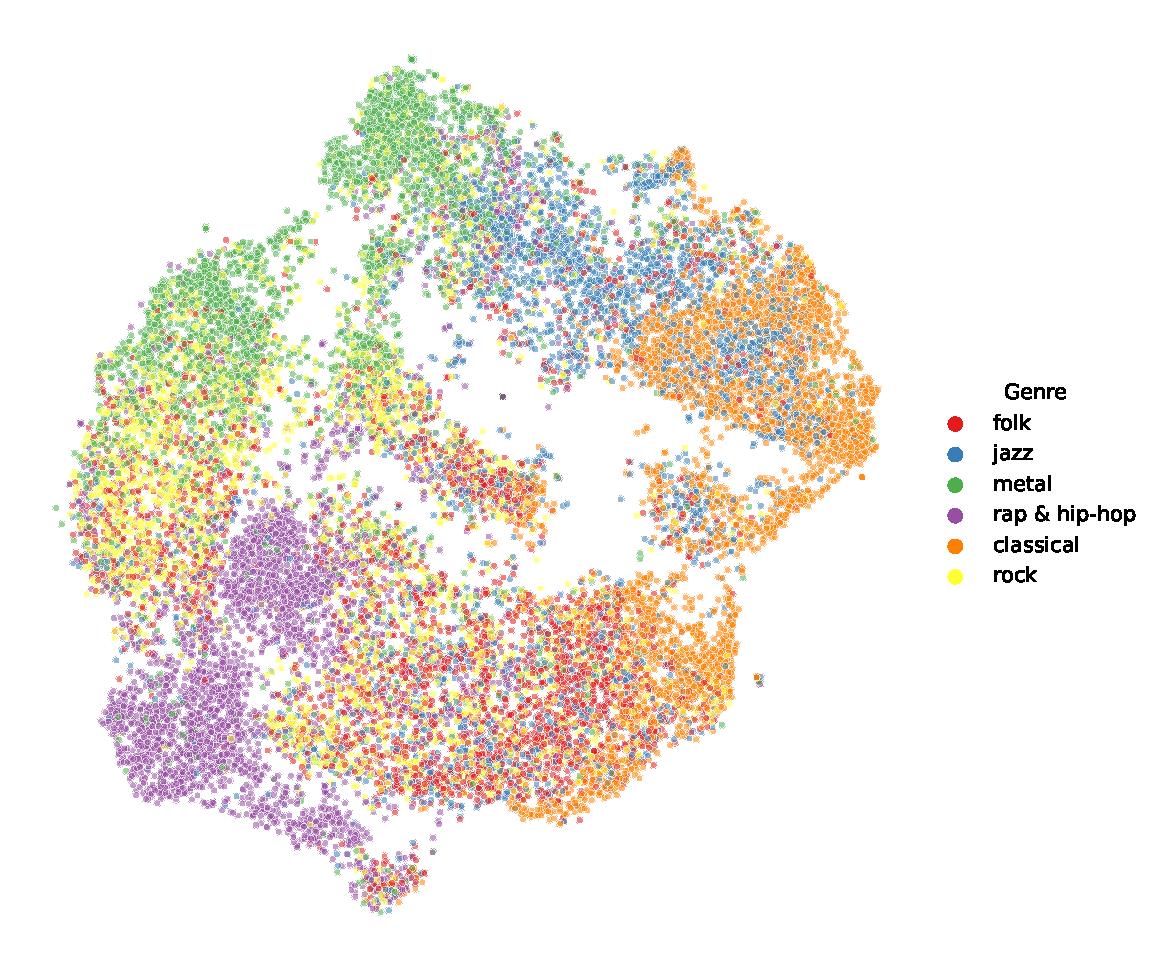
\includegraphics[width=1.0\textwidth]{../figures/tsne_genres.pdf}
%   \caption{Two-dimensional embedding of song features results in distinct clusters corresponding to musical supergenres.}
%   \label{fig:tsne_genres}
% \end{figure}

% \end{appendix}

\end{document}
